\documentclass[ngerman,abstract=true]{scrartcl}
\usepackage{babel}
\usepackage{csquotes}

% typography
\usepackage{fontspec}
\setmainfont{Open Sans}[
  BoldFont={Open Sans Bold},
  ItalicFont={Open Sans Italic}]
\setsansfont{Open Sans}[
  BoldFont={Open Sans Bold},
  ItalicFont={Open Sans Italic}]
\setmonofont{Menlo}
\usepackage[factor=2000]{microtype}

% graphics, drawings, etc.
\usepackage{xcolor}
\usepackage{graphicx}
\usepackage[most]{tcolorbox}
\usepackage{tikz}
\usetikzlibrary{shapes.geometric}
\usetikzlibrary{shapes.arrows}
\usetikzlibrary{positioning}
\usetikzlibrary{matrix}
\newtcolorbox{anmerkung}{%
  grow to left by=10pt,
  colback=black!10,
  colframe=white,
  coltitle=black,
  borderline west={4pt}{0pt}{black!30},
  boxrule=0pt,
  boxsep=0pt,
  %breakable,
  enhanced jigsaw,
  title={Anmerkung\par},
  fonttitle={\bfseries},
  attach title to upper={}}

% highlighting, lists, code
\usepackage{soul}
\usepackage{enumitem}
\usepackage{listings}
\lstset{
  basicstyle=\ttfamily,
  escapeinside=||,
  keywordstyle=\color{blue!50!black},
  stringstyle=\color{green!50!black}}

% nice tables
\usepackage{booktabs,array}
\newcommand{\tablespacing}[1]{\renewcommand{\arraystretch}{#1}}

% links
\usepackage[
  colorlinks,
  linkcolor={red!50!black},
  citecolor={blue!50!black},
  urlcolor={blue!80!black}
]{hyperref}

\title{Betriebssysteme}
\date{Wintersemester 2018-2019}
\author{Prof.\ Neeraj Suri, Dr.\ Stefan Winter}

\begin{document}
\maketitle
  
\tableofcontents
\newpage
  
\section{Geschichte}

Am Anfang gab es noch keine Betriebssysteme, alle Programme liefen direkt auf der Hardware (\emph{Bare Metal}). Da jedes Programm in irgendeiner Weise Daten verarbeiten muss, musste man für jedes Programm gewisse Eingaben zugänglich machen, und gewisse Ausgaben in einer für dem Benutzer nutzbaren Art ausgeben. Also musste man Code schreiben, der eigentlich garnichts mit dem Programm zu tun hat, sondern nur dazu dient, diese Eingaben und Ausgaben zu ermöglichen.

\begin{figure}[h]\centering
\begin{tikzpicture}[
  code/.style={rectangle, draw, rounded corners, text width=5.5cm, align=left}]
\node[code,label={\textbf{Code}}] (code) {\verb|get_user_input();|\\\verb|do_processing();|\\\verb|generate_user_output();|};
\node[label=below:{\textbf{Output}}] (screen) at (-4,-3) {
\includegraphics[width=3cm]{media/screen}};
\node[label=below:{\textbf{Input}}] (input) at (0,-3) {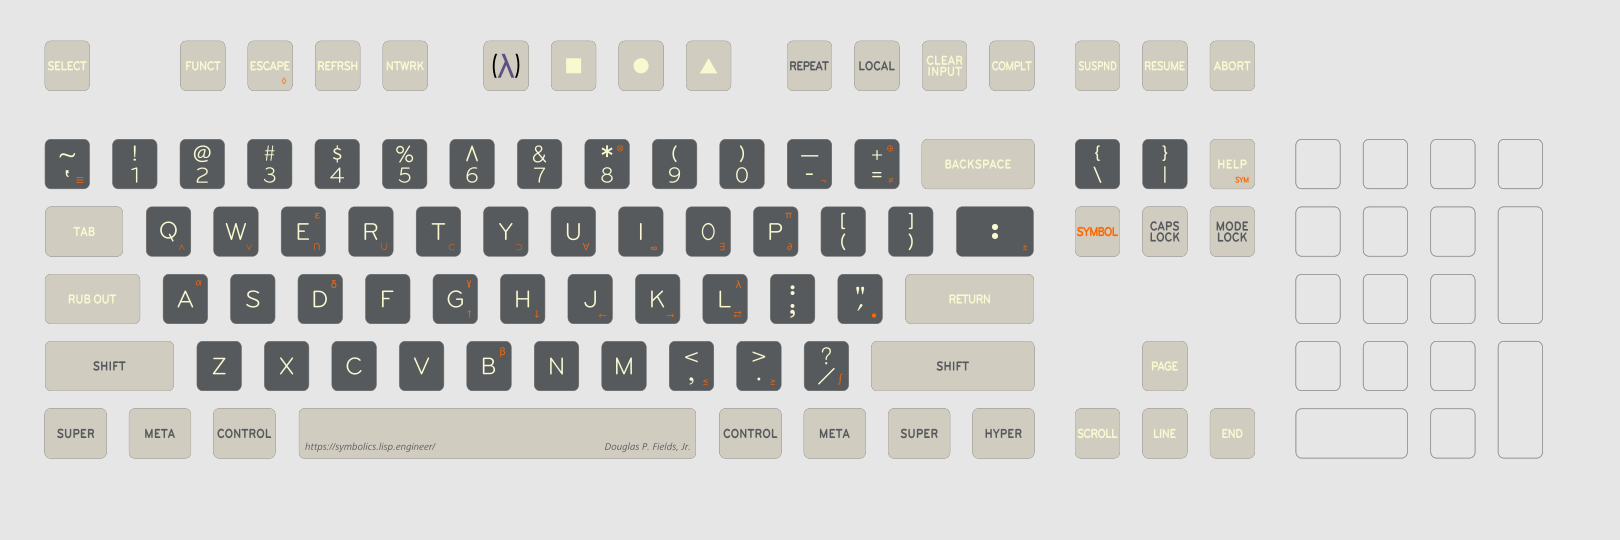
\includegraphics[width=4cm]{media/keyboard}};
\node[label=below:{\textbf{Storage}}] (storage) at (4,-3) {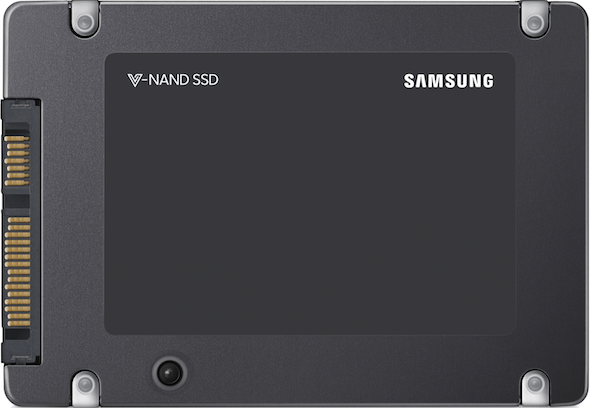
\includegraphics[width=3cm]{media/ssd}};
\draw[<->] (code) -- ++(-4,0) -- (screen);
\draw[->] (code) -- (input);
\draw[->] (code) -- ++(4,0) -- (storage);
\end{tikzpicture}
\caption{Programmierung auf Hardware ohne Abstraktion}\label{fig:prog}
\end{figure}

\subsection{Library}

Irgendwann erkannte man dann, dass man sehr oft gewisse Funktionalität neu implementieren musste, weil unterschiedliche Programme ähnliche Eingaben erwarteten oder ähnliche Ausgaben erzeugten, und man diesen Code dafür widerholte. Eine Idee hier ist, den Code, den man häufig verwendet, in eine \emph{Library} packt. Damit können diese Routinen wiederverdendet werden. Außerdem können Programme sich so mehr auf ihre eigentlichen Aufgaben konzentrieren.

\begin{figure}[h]\centering
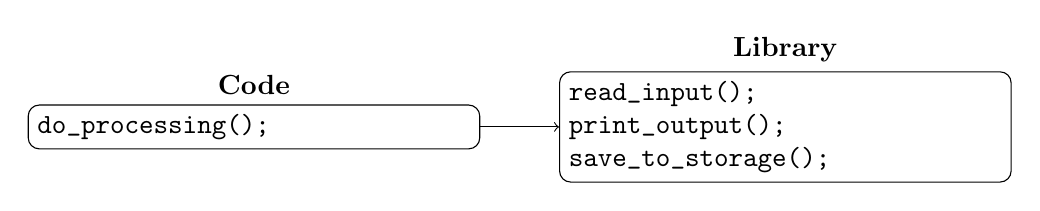
\begin{tikzpicture}[
  code/.style={rectangle, draw, rounded corners, text width=5.5cm, align=left}]
\node[code,label={\textbf{Code}}] (code) {\verb|do_processing();|};
\node[code,label={\textbf{Library}},right=of code] (library) {\verb|read_input();|\\\verb|print_output();|\\\verb|save_to_storage();|};
\draw[->] (code) -- (library);
\end{tikzpicture}
\caption{Ausbau von Funktionen in eine Library}\label{fig:library}
\end{figure}

Der Nachteil von diesem Ansatz war, dass diese Libraries immer wieder umgeschrieben mussten, wenn ein anderer Computer verwendet wurde.

\subsection{Exponentielles Wachstum von Hardwarekomplexität}

\begin{figure}\centering
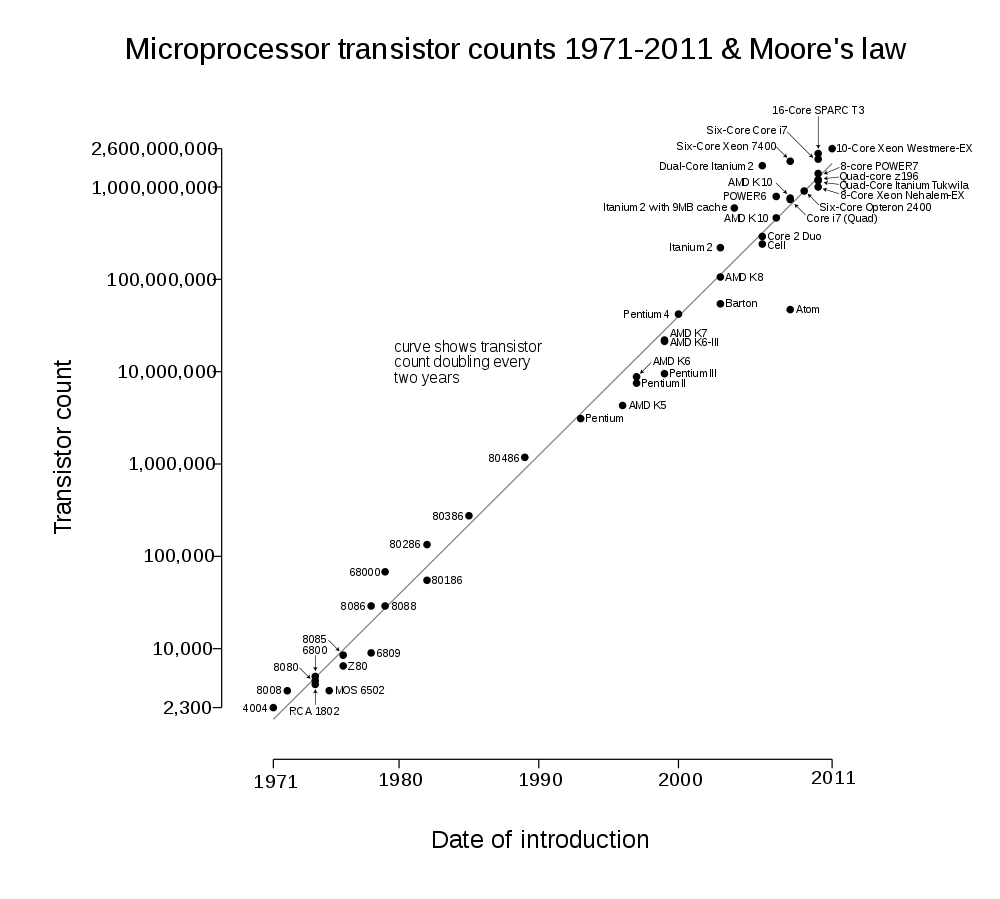
\includegraphics[trim={1.8cm 1.8cm 1cm 3.6cm},clip,width=0.8\linewidth]{media/mooreslaw}
\caption{Hardwarekomplexitätswachstum seit 1971.}\label{fig:mooreslaw}
\end{figure}

Es ergab sich also die Schwierigkeit, dass die Hardware sich so rasant entwickelt. Dies ist in Abbildung \ref{fig:mooreslaw} graphisch aufgezeigt, wobei man anmerken muss, dass die Skala logarithmisch ist. Das scheinbar lineare Wachstum der Transistoranzahl ist also tatsächlich ein exponentielles. Das nennt man auch Moore's law, nach dem Begründer von Intel.

\subsection{Heute}

\begin{figure}[p]\centering
\begin{tikzpicture}
\node (phone) {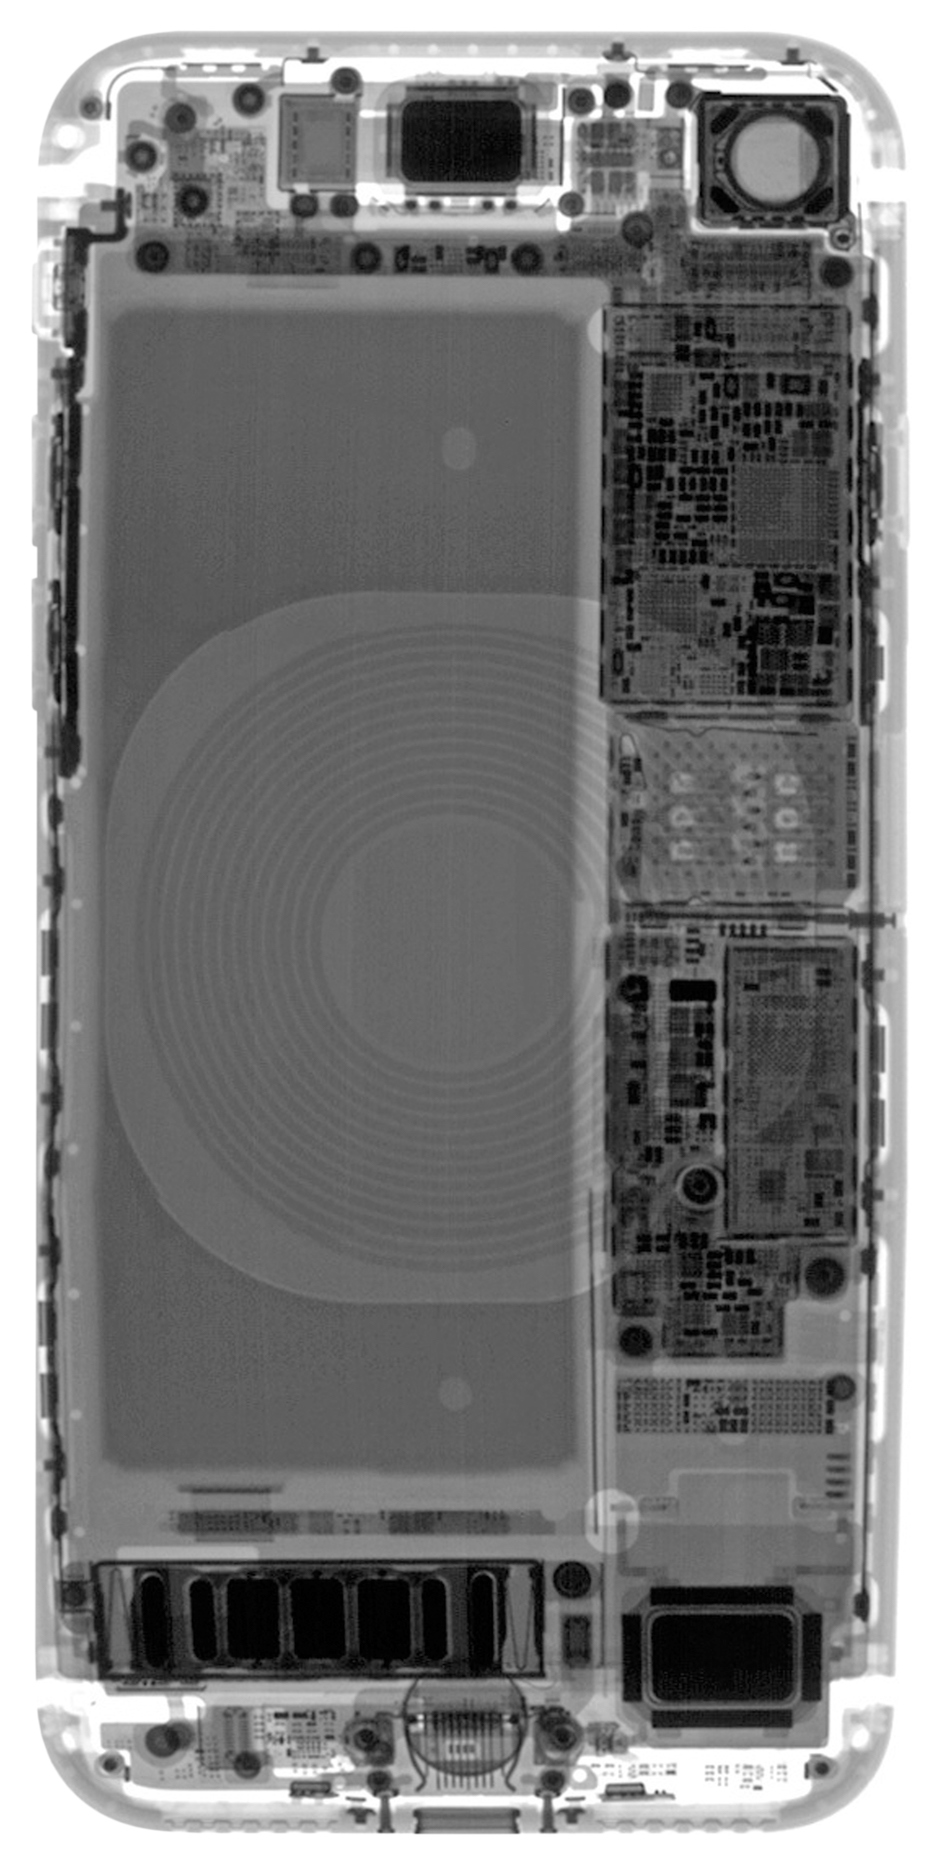
\includegraphics[width=8cm]{media/phone}};
\draw[very thick, white] (1.3,3.1) rectangle (3.2,4.9) node[pos=.5] {\textbf{A11}};
\draw[very thick, white] (1.3,2.1) rectangle +(1,0.9) node[pos=.5] {\textbf{QM}};
\draw[very thick, white] (2.1,-0.8) rectangle +(1.1,0.8) node[pos=.5] {\textbf{SW}};
\node[text width=6cm,align=left] (a11) at (7,6) {\textbf{Apple A11 SoC}\\Betriebssystem: iOS (Darwin), UNIX-Derivat, POSIX kompatibel.};
\node[below=5mm of a11, text width=6cm,align=left] (se) {\textbf{Apple Secure Enclave}\\Im A11-Chip eingebaut\\Betriebssystem: Basiert auf dem L4 Mikrokernel};
\node[below=5mm of se, text width=6cm,align=left] (qc) {\textbf{Qualcomm Snapdragon X16}\\LTE Modem\\Betriebssystem: Unbekanntes RTOS, eventuell REX OS};
\node[below=5mm of qc, text width=6cm,align=left] (skyone) {\textbf{Skyworks SkyOne SKY78140}\\CDMA Modem\\Betriebssystem: Unbekannt};
\end{tikzpicture}
\caption{Betriebssyteme auf Konsumergeräten am Beispiel iPhone}\label{fig:osdevices}
\end{figure}
\begin{figure}[p]\centering
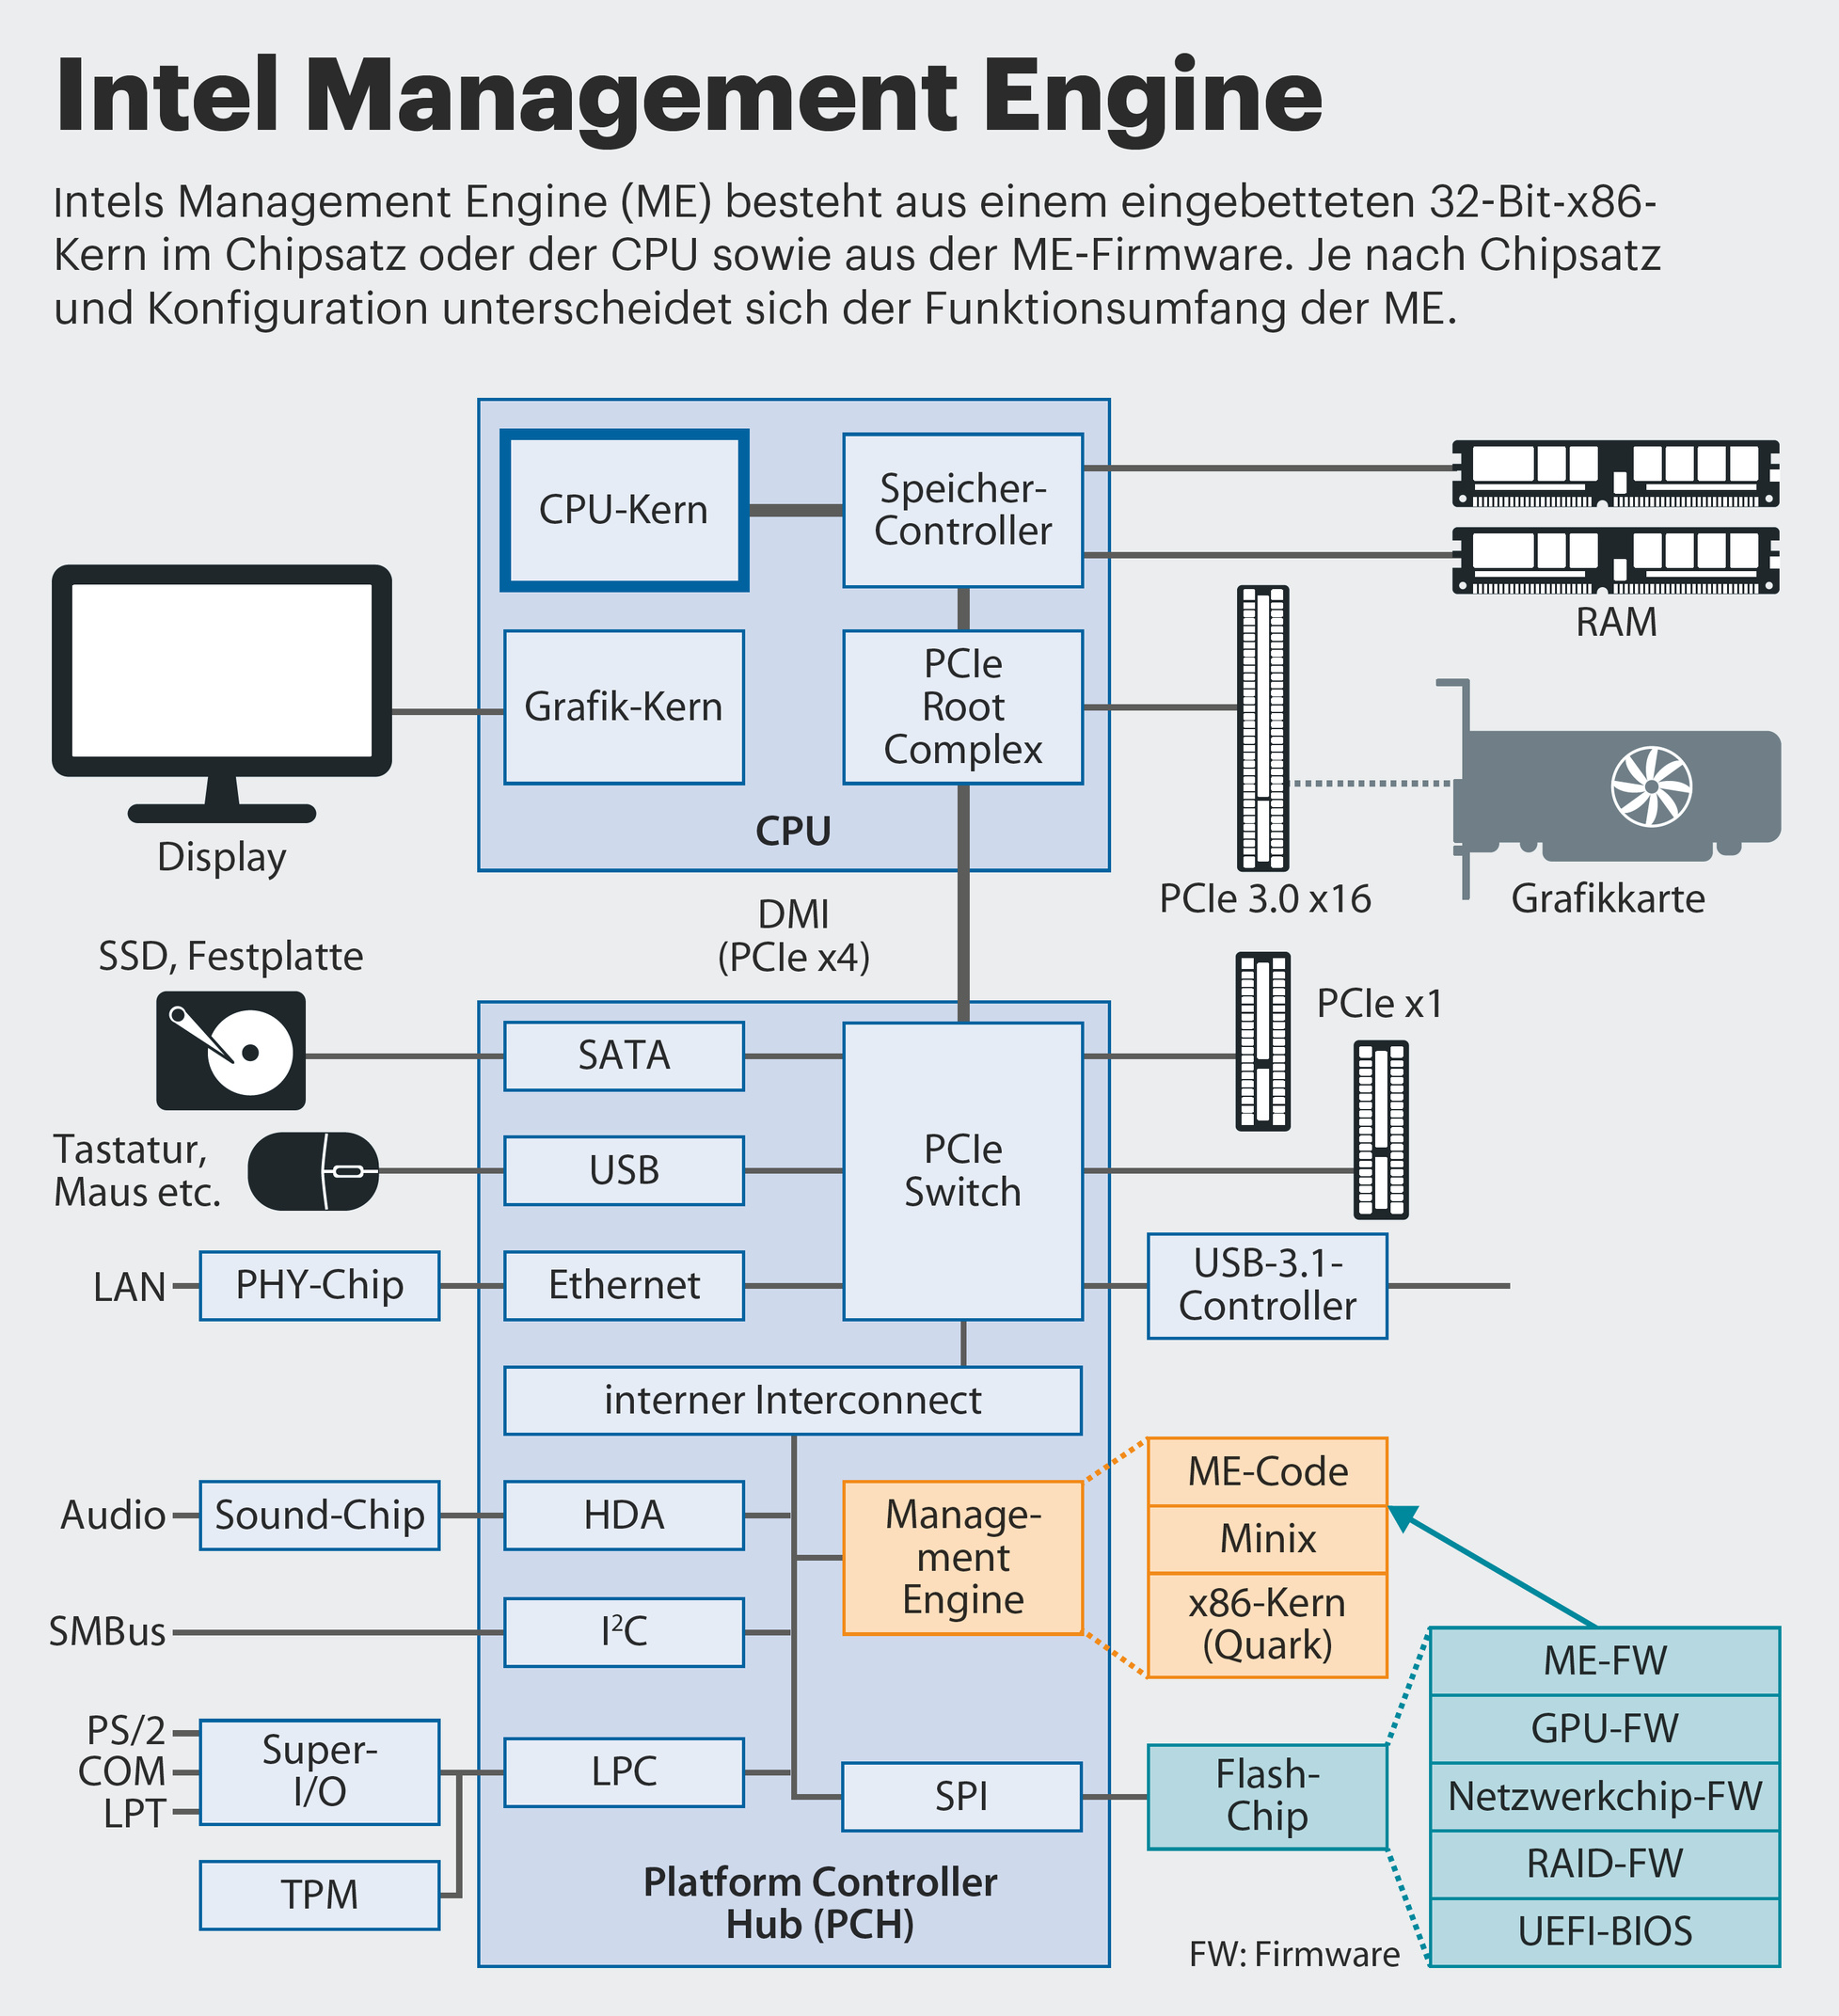
\includegraphics[width=0.8\textwidth]{media/intelme}
\caption{Intel Management Engine. Quelle: Heise.de}\label{fig:intelme}
\end{figure}

Heutzutage sind Betriebssysteme \emph{überall}. Von Fernsehehern zu Autos, Servern, Handys bis hin zu Operationssälen. Interessanterweise sind teilweise mehrere Betriebssysteme auf einem Gerät zu finden. Abbildungen \ref{fig:osdevices} und \ref{fig:intelme} zeigen, dass sogar in den Geräten, die wir tagtäglich verwenden, oft mehr steckt, als wir denken.

Die Betriebssysteme, die wir benutzen, haben oft sehr viele Features eingebaut. 

\section{Definition}

Wie definiert man eigentlich, was ein Betriebssystem ist, und was nicht? Dazu gibt es nicht nur eine, sondern gleich mehrere Definitionen. 

\subsection{Hardwareabstraktion}

Man kann ein Betriebssystem als eine Hardwareabstraktionsschicht beschreiben. Das Betriebssytem ist als dafür zuständig, eine Ausführungsumgebung zu erstellen für die Programme, die darauf laufen sollen. Dazu muss das Betriebssystem den Programmen eine Abstraktionsebene bieten, damit diese nicht direkt mit der Hardware interagieren müssen. Außerdem muss das Betriebssyste die Resourcen verwalten und (idealerweise fair) zwischen den Programmen teilen.

Wenn man sich jetzt mal anschaut, wie viel Code eigentlich hinter der Ausführung eines kleinen, simplen Programms steckt, dann merkt man, wie viel eigentlich hinter den Kulissen passieren muss, damit die Programme das tun, was wir von ihnen erwarten. In Abbildung \ref{fig:hardwareabstraktion} ist zu sehen, welche Ebenen eigentlich unter einen Programm liegen, und wie viel Code diese Beinhalten.
\begin{figure}[!h]\centering\tablespacing{1.4}
\begin{tabular}{@{}p{3.4cm}p{2.6cm}r@{}}
\toprule
\textbf{Ebene} & \textbf{Beispiel} & \textbf{Zeilen}\\
\midrule
Java Bytecode 
  & & \textasciitilde 1\,000\\
Java Runtime 
  & \verb|openjdk11| & 8\,047\,913\\
Support Libraries 
  & \verb|glib| & 460\,641\\
  & \verb|libcxx| & 441\,343\\
System Libraries 
  & \verb|glibc| & 1\,384\,092\\
Kernel 
  & \verb|darwin| & 1\,070\,917\\
  & \verb|openbsd| & 2\,235\,267\\
  & \verb|netbsd| & 16\,735\,800\\
  & \verb|linux| & 17\,120\,205\\
  & \verb|windows| & \textasciitilde 65\,000\,000\\
Hardware &&\\
\bottomrule 
\end{tabular}
\caption{Hardwareabstraktionsebenen und Codegröße}\label{fig:hardwareabstraktion}
\end{figure}

\begin{anmerkung}
Ich habe mir mal die Freiheit genommen, die Zeilen Sourcecode für die meisten Projekte hier durchzuzählen. Dazu habe ich das Programm \verb|cloc| benutzt (auf macOS mit \verb|brew install cloc| installierbar). Die \verb|libcxx| ist die C++ Standard Library, die vom Clang Compiler des LLVM Projekt genutzt wird (wird verwendet von iOS, macOS, Linux, usw.). Der macOS Kernel, \verb|darwin|, ist Quelloffen, deswegen habe ich den auch mitgenommen. Allerdings muss man dazu sagen, dass dieser modular aufgebaut ist, und hier keine Module mitgenommen wurden, deswegen sind die Resultate nicht direkt verlgeichbar. Bei den BSDs habe ich den \emph{gesamten} Quelltext ausgewertet, das behinhaltet aber auch Code, der nicht unbedingt im Kernel steckt.
\end{anmerkung}


Außerdem musste man ja.

\end{document}










